\documentclass[tikz,border=3pt]{standalone}
\usepackage[T1]{fontenc}
\usepackage{amsmath}
\usepackage{XCharter}
\usepackage[xcharter]{newtxmath}
\usepackage[scaled=.92]{helvet}
\usepackage{pgfplots}
\usetikzlibrary{arrows.meta,positioning,fit,calc,backgrounds,decorations.pathreplacing,patterns}
\usepgfplotslibrary{groupplots,fillbetween}
\pgfplotsset{compat=1.18}
\definecolor{ink}{HTML}{172536}
\definecolor{rgb}{HTML}{3563B8}
\definecolor{event}{HTML}{17857C}
\definecolor{fusion}{HTML}{76529C}
\definecolor{reference}{HTML}{8994A3}
\definecolor{warn}{HTML}{AC5948}
\definecolor{muted}{HTML}{657183}
\definecolor{rule}{HTML}{D9E0E8}
\definecolor{pale}{HTML}{F5F7FA}
\color{ink}
\tikzset{box/.style={rounded corners=2pt,draw=rule,fill=white,align=center,inner sep=4pt,font=\sffamily\fontsize{9}{10.8}\selectfont,minimum height=9mm},rb/.style={box,draw=rgb!50,fill=rgb!5},eb/.style={box,draw=event!50,fill=event!5},fb/.style={box,draw=fusion!55,fill=fusion!5},arrow/.style={-{Latex[length=1.8mm]},line width=.65pt,draw=muted},note/.style={font=\sffamily\fontsize{8.4}{10.2}\selectfont,align=center,text=muted},heading/.style={font=\sffamily\fontsize{10}{12}\selectfont\bfseries,align=left,text=ink}}
\pgfplotsset{paper/.style={width=15.7cm,height=6cm,axis lines*=left,axis line style={rule},tick style={draw=none},tick label style={font=\sffamily\fontsize{8.8}{10.4}\selectfont,text=muted},label style={font=\sffamily\fontsize{9.4}{11}\selectfont,text=ink},title style={font=\sffamily\fontsize{10}{12}\selectfont\bfseries,text=ink},legend style={draw=none,fill=none,font=\sffamily\fontsize{9}{11}\selectfont,cells={anchor=west}},grid=major,grid style={rule!65,line width=.3pt},minor tick num=0,scaled ticks=false,unbounded coords=jump,clip mode=individual}}
\begin{document}
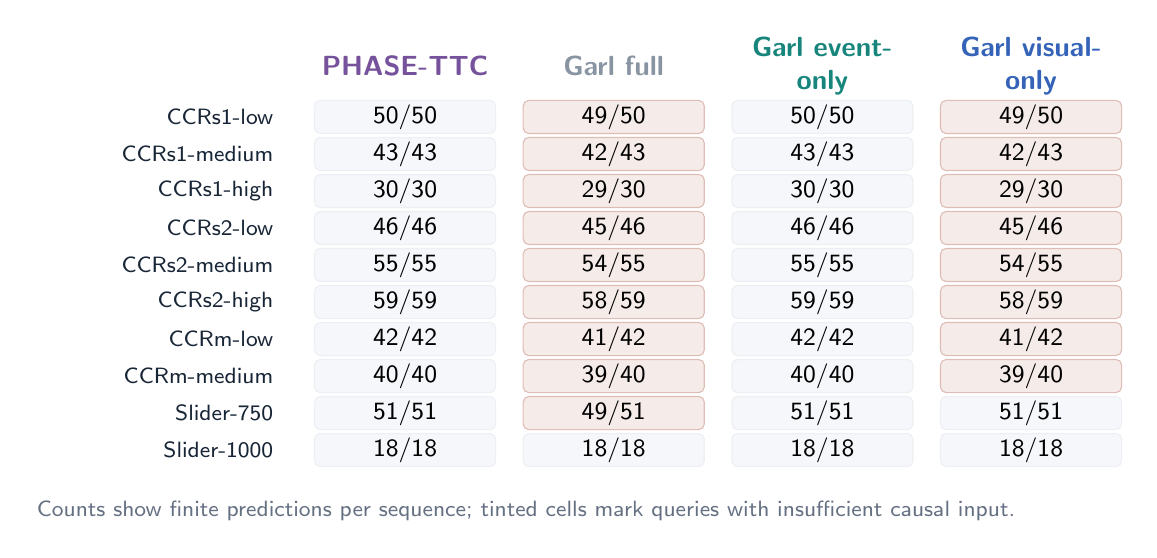
\begin{tikzpicture}[x=1cm,y=1cm]
\node[heading,text=fusion,text width=2.25cm,align=center] at (5.0,5.5) {PHASE-TTC};
\node[heading,text=reference,text width=2.25cm,align=center] at (7.65,5.5) {Garl full};
\node[heading,text=event,text width=2.25cm,align=center] at (10.3,5.5) {Garl event-only};
\node[heading,text=rgb,text width=2.25cm,align=center] at (12.95,5.5) {Garl visual-only};
\node[note,anchor=east,text=ink] at (3.45,4.85) {CCRs1-low};
\node[box,minimum width=2.3cm,minimum height=4.2mm,inner sep=1pt,fill=pale,draw=rule!50] at (5.0,4.85) {50/50};
\node[box,minimum width=2.3cm,minimum height=4.2mm,inner sep=1pt,fill=warn!12,draw=warn!40] at (7.65,4.85) {49/50};
\node[box,minimum width=2.3cm,minimum height=4.2mm,inner sep=1pt,fill=pale,draw=rule!50] at (10.3,4.85) {50/50};
\node[box,minimum width=2.3cm,minimum height=4.2mm,inner sep=1pt,fill=warn!12,draw=warn!40] at (12.95,4.85) {49/50};
\node[note,anchor=east,text=ink] at (3.45,4.38) {CCRs1-medium};
\node[box,minimum width=2.3cm,minimum height=4.2mm,inner sep=1pt,fill=pale,draw=rule!50] at (5.0,4.38) {43/43};
\node[box,minimum width=2.3cm,minimum height=4.2mm,inner sep=1pt,fill=warn!12,draw=warn!40] at (7.65,4.38) {42/43};
\node[box,minimum width=2.3cm,minimum height=4.2mm,inner sep=1pt,fill=pale,draw=rule!50] at (10.3,4.38) {43/43};
\node[box,minimum width=2.3cm,minimum height=4.2mm,inner sep=1pt,fill=warn!12,draw=warn!40] at (12.95,4.38) {42/43};
\node[note,anchor=east,text=ink] at (3.45,3.9099999999999997) {CCRs1-high};
\node[box,minimum width=2.3cm,minimum height=4.2mm,inner sep=1pt,fill=pale,draw=rule!50] at (5.0,3.9099999999999997) {30/30};
\node[box,minimum width=2.3cm,minimum height=4.2mm,inner sep=1pt,fill=warn!12,draw=warn!40] at (7.65,3.9099999999999997) {29/30};
\node[box,minimum width=2.3cm,minimum height=4.2mm,inner sep=1pt,fill=pale,draw=rule!50] at (10.3,3.9099999999999997) {30/30};
\node[box,minimum width=2.3cm,minimum height=4.2mm,inner sep=1pt,fill=warn!12,draw=warn!40] at (12.95,3.9099999999999997) {29/30};
\node[note,anchor=east,text=ink] at (3.45,3.4399999999999995) {CCRs2-low};
\node[box,minimum width=2.3cm,minimum height=4.2mm,inner sep=1pt,fill=pale,draw=rule!50] at (5.0,3.4399999999999995) {46/46};
\node[box,minimum width=2.3cm,minimum height=4.2mm,inner sep=1pt,fill=warn!12,draw=warn!40] at (7.65,3.4399999999999995) {45/46};
\node[box,minimum width=2.3cm,minimum height=4.2mm,inner sep=1pt,fill=pale,draw=rule!50] at (10.3,3.4399999999999995) {46/46};
\node[box,minimum width=2.3cm,minimum height=4.2mm,inner sep=1pt,fill=warn!12,draw=warn!40] at (12.95,3.4399999999999995) {45/46};
\node[note,anchor=east,text=ink] at (3.45,2.9699999999999998) {CCRs2-medium};
\node[box,minimum width=2.3cm,minimum height=4.2mm,inner sep=1pt,fill=pale,draw=rule!50] at (5.0,2.9699999999999998) {55/55};
\node[box,minimum width=2.3cm,minimum height=4.2mm,inner sep=1pt,fill=warn!12,draw=warn!40] at (7.65,2.9699999999999998) {54/55};
\node[box,minimum width=2.3cm,minimum height=4.2mm,inner sep=1pt,fill=pale,draw=rule!50] at (10.3,2.9699999999999998) {55/55};
\node[box,minimum width=2.3cm,minimum height=4.2mm,inner sep=1pt,fill=warn!12,draw=warn!40] at (12.95,2.9699999999999998) {54/55};
\node[note,anchor=east,text=ink] at (3.45,2.5) {CCRs2-high};
\node[box,minimum width=2.3cm,minimum height=4.2mm,inner sep=1pt,fill=pale,draw=rule!50] at (5.0,2.5) {59/59};
\node[box,minimum width=2.3cm,minimum height=4.2mm,inner sep=1pt,fill=warn!12,draw=warn!40] at (7.65,2.5) {58/59};
\node[box,minimum width=2.3cm,minimum height=4.2mm,inner sep=1pt,fill=pale,draw=rule!50] at (10.3,2.5) {59/59};
\node[box,minimum width=2.3cm,minimum height=4.2mm,inner sep=1pt,fill=warn!12,draw=warn!40] at (12.95,2.5) {58/59};
\node[note,anchor=east,text=ink] at (3.45,2.03) {CCRm-low};
\node[box,minimum width=2.3cm,minimum height=4.2mm,inner sep=1pt,fill=pale,draw=rule!50] at (5.0,2.03) {42/42};
\node[box,minimum width=2.3cm,minimum height=4.2mm,inner sep=1pt,fill=warn!12,draw=warn!40] at (7.65,2.03) {41/42};
\node[box,minimum width=2.3cm,minimum height=4.2mm,inner sep=1pt,fill=pale,draw=rule!50] at (10.3,2.03) {42/42};
\node[box,minimum width=2.3cm,minimum height=4.2mm,inner sep=1pt,fill=warn!12,draw=warn!40] at (12.95,2.03) {41/42};
\node[note,anchor=east,text=ink] at (3.45,1.5599999999999996) {CCRm-medium};
\node[box,minimum width=2.3cm,minimum height=4.2mm,inner sep=1pt,fill=pale,draw=rule!50] at (5.0,1.5599999999999996) {40/40};
\node[box,minimum width=2.3cm,minimum height=4.2mm,inner sep=1pt,fill=warn!12,draw=warn!40] at (7.65,1.5599999999999996) {39/40};
\node[box,minimum width=2.3cm,minimum height=4.2mm,inner sep=1pt,fill=pale,draw=rule!50] at (10.3,1.5599999999999996) {40/40};
\node[box,minimum width=2.3cm,minimum height=4.2mm,inner sep=1pt,fill=warn!12,draw=warn!40] at (12.95,1.5599999999999996) {39/40};
\node[note,anchor=east,text=ink] at (3.45,1.0899999999999999) {Slider-750};
\node[box,minimum width=2.3cm,minimum height=4.2mm,inner sep=1pt,fill=pale,draw=rule!50] at (5.0,1.0899999999999999) {51/51};
\node[box,minimum width=2.3cm,minimum height=4.2mm,inner sep=1pt,fill=warn!12,draw=warn!40] at (7.65,1.0899999999999999) {49/51};
\node[box,minimum width=2.3cm,minimum height=4.2mm,inner sep=1pt,fill=pale,draw=rule!50] at (10.3,1.0899999999999999) {51/51};
\node[box,minimum width=2.3cm,minimum height=4.2mm,inner sep=1pt,fill=pale,draw=rule!50] at (12.95,1.0899999999999999) {51/51};
\node[note,anchor=east,text=ink] at (3.45,0.6200000000000001) {Slider-1000};
\node[box,minimum width=2.3cm,minimum height=4.2mm,inner sep=1pt,fill=pale,draw=rule!50] at (5.0,0.6200000000000001) {18/18};
\node[box,minimum width=2.3cm,minimum height=4.2mm,inner sep=1pt,fill=pale,draw=rule!50] at (7.65,0.6200000000000001) {18/18};
\node[box,minimum width=2.3cm,minimum height=4.2mm,inner sep=1pt,fill=pale,draw=rule!50] at (10.3,0.6200000000000001) {18/18};
\node[box,minimum width=2.3cm,minimum height=4.2mm,inner sep=1pt,fill=pale,draw=rule!50] at (12.95,0.6200000000000001) {18/18};
\node[note,anchor=west] at (.2,-.15) {Counts show finite predictions per sequence; tinted cells mark queries with insufficient causal input.};\end{tikzpicture}
\end{document}
